\documentclass[a4paper,10pt]{article}
\usepackage[utf8]{inputenc}
\usepackage{graphicx}
\usepackage{hyperref}
\usepackage{minted}
%opening
\title{The Memory \& Storage Design of Neo4J}
\author{Fabian Klopfer}

\begin{document}

\maketitle

\begin{abstract}
In this document I describe the internals of the storage layer of the popular native graph database Neo4J. A detailed description of how records are stored into which files and how these are accessed is to be elaborated on in the following article. This is a translation, update and extension of previous work done by Michael Brendle. 
\end{abstract}



\section{Introduction}
Relational databases store tables of data. The links considered in this category of DBMS are mostly used to stitch together the fields of an entry into one row again, after it has been split to satisfy a certain normal form. Of course one may also store tables where one table stores nodes and the other table's fields are node IDs to represent relationships.

However, in order to traverse the graph, one has either to do a lot of rather expensive look ups or store auxiliary structures to speed up the look up process. In particular when using B-trees as index structure, each look up takes $\mathcal{O}(\log(n))$ steps to locate a specific edge. Alternatively one could store an additional table that holds edge lists such that the look up of outgoing or incomming edges is only $\mathcal{O}(\log(n))$ which would speed up breadth first traversals. But still one has to compute joins in order to continue the traversal in terms of depth. Another way to speed things up is to use a hash-based index, but this also has a certain overhead aside from the joins.

In contrast to relational data base management systems, native graph databases use structures specialised for this kind of queries. In the remainder of the document I discuss based upon Michael Brendle's work what structures and mechanisms the graph database Neo4J uses in order to achieve this superior performance in the domain of graphs.

First of all, let us consider the high level architecture of a database management systems as shown in figure~\ref{dbms_arch} --- with a focus on the storage and loading elements.

\begin{figure}[htp]\label{dbms_arch}
 \begin{center}
  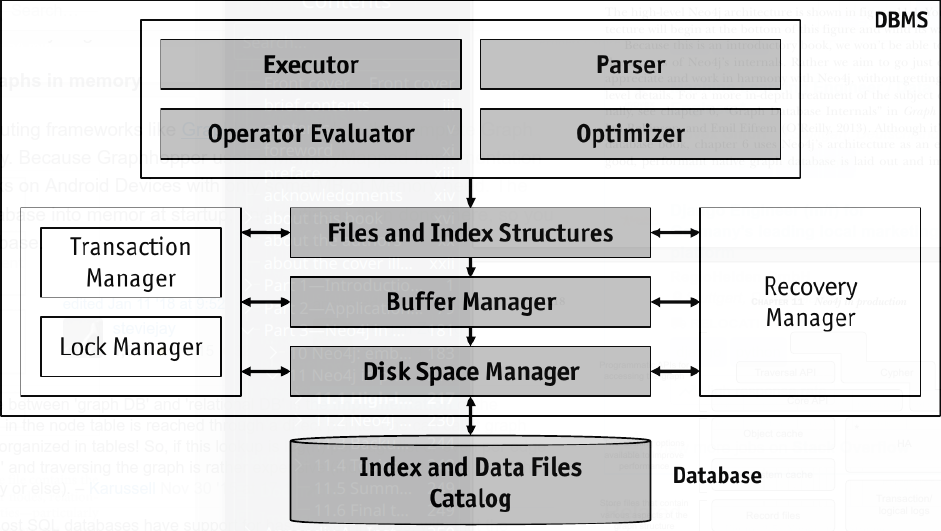
\includegraphics[keepaspectratio,width=0.7\textwidth]{img/RDBMS.png}
 \end{center}
 \caption{The typical structure of a relational database management system } %TODO citation
\end{figure}

Here The disk space manager, sometimes also called storage manager, handles de-/allocations, reads \& writes and provides the concept of a page: A disk block brought into memory. For that it needs to keep track of free blocks in the allocated file. Optimally both a disk block and a page are of the same size. One crucial task of a disk space manager is to store sequences of pages into continuous memory blocks in order to optimize data locality. Data locality has the upside, that one needs only one I/O operation to load multiple pages. To summarize the two most important objectives of a storage manager are to provide a locality-preserving mapping from pages to blocks based upon the information in the DBMS and to abstract physical storage to pages, taking care of allocation and access.
A buffer manager is used to mediate between external storage and main memory. It maintains a designated pre-allocated area of main memory --- called the buffer pool --- to load, cache and evict pages into or from main memory. It's objective is to minimize the number of disk reads to be executed by caching, pre-fetching and the usage of suitable replacement policies. It also needs to take care of allocating a certain fraction of pages to each transaction.

The final memory and storage model relevant component of the  of a database management system is the file layout and possible index structures. 
In order to store data a DBMS may either store one single or multiple files to maintain records. 

A file may consist of a set of pages containing a set of slots. A slot stores one record with each record containing a set of fields. Further the database needs to keep track of free space in the file: A linked list or a directory must record free pages and some structure needs to keep track of the free slots either globally or per page. 

Records may be of fixed or of variable size, depending on the types of their fields. Records can be layout in row or column major order. That is one can store sequences of tuples or sequences of fields. The former is beneficial if a lot of update, insert or delete operations are committed to the database, while the latter optimizes the performance when scans and aggregations are the most typical queries to the system.

Another option is to store the structure of the records along with pointers to the values of their fields in one files and the actual values in one or multiple separate files. Also distinct types of tables can be stored in different files. For example entities and relations can be stored in different files with references to each other, thus enabling the layout of these two to be specialized to their structure and usage in queries.

Files may either organize their records in random order (heap file), sorted or using a hash function on one or more fields. All of these approaches have upsides and downsides when it comes to scans, searches, insertions, deletions and updates. 

To mitigate the effect that result from selecting one file organization or another, the concept of indexes have been introduced. Indexes are auxiliary structures to speed up certain operations that depend on one field. Indexes may be clustered or unclustered. An index over field $F$ is called clustered if the underlying data file is sorted according to the values of $F$. An unclustered index over field $G$ is one where the file is not sorted according to $G$. In a similar way indexes can be sparse or dense. A sparse index has less index entries than records, mostly one index entry per file. This can of course only be done for clustered indexes as the sorting of the data file keeps the elements between index keys in order. An index is dense if there is a one to one correspondence between records and index entries. There are different variants of storing index entries which have again certain implications on the compactness of the index and the underlying design decisions.

In another view of database management systems architectures, this boils down to the design decisions one has to make when implementing the storage layer and the access layer as shown in figure~\ref{dbms_arch_layers}.

\begin{figure}[htp]\label{dbms_arch_layers}
 \begin{center}
  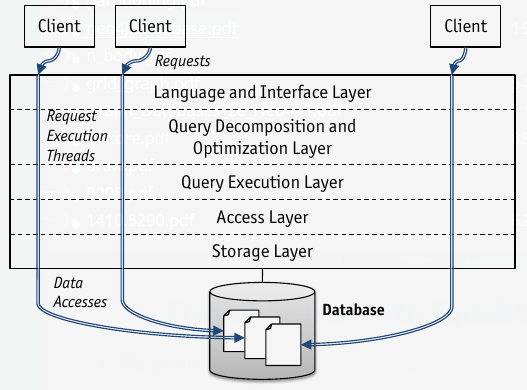
\includegraphics[keepaspectratio,width=0.6\textwidth]{img/layered_RDBMS.png}
 \end{center}
 \caption{The architecture of a database management system from another point of view.} %TODO citation
\end{figure}

Here the storage layer is in close correspondence to the disk space manager in combination with the buffer manager, while the files and index structures provide the access layer.

All these considerations make choosing different file splits, layouts, orderings, addressing schemes, management structures, de-/allocation schemes and indexes a complex set of dependent choices. 
These depend mainly on the structure of the data to be stored and the queries to be run. 

When restricting to graph structures where nodes and relationships are allowed to have properties and labels and types respectively, this allows one to narrow down some of the design decisions. In particular the example of a popular graph native database --- Neo4J --- is what I discuss in the next sections. 

To get an overview of the architecture let us consider figure~\ref{N4J_HLA_Emil}. 

\begin{figure}[htp]\label{N4J_HLA_Emil}
 \begin{center}
  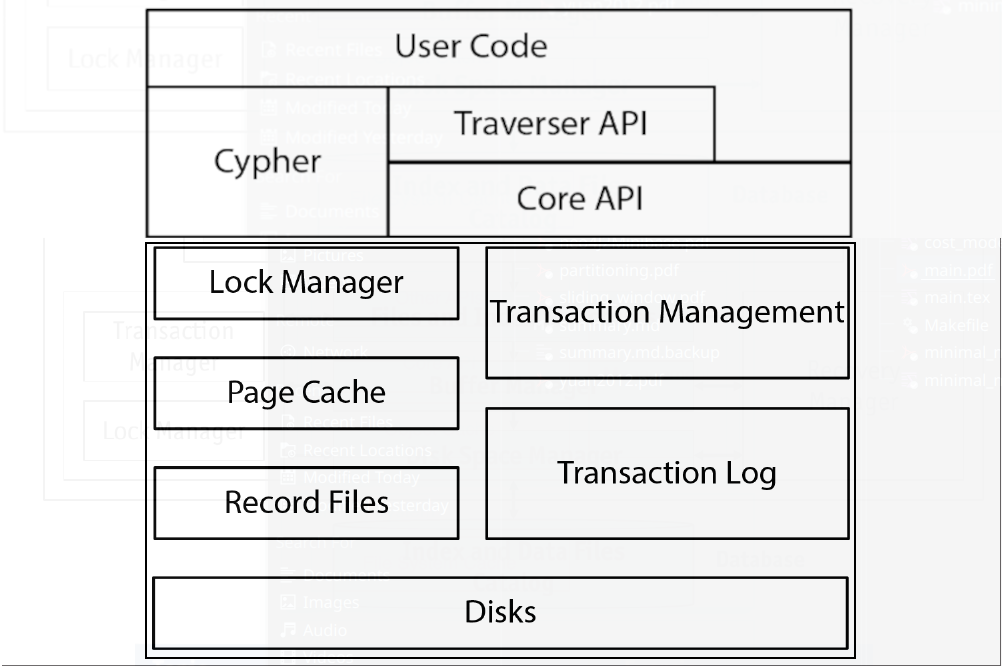
\includegraphics[keepaspectratio,width=0.6\textwidth]{img/N4J_HLA_Emil.png}
 \end{center}
 \caption{The high level architecture of Neo4J according to Emil Efrim, the co-founder of Neo technologies.} %TODO citation
\end{figure}

Here we can see that the previous schema is not exactly straight forward to apply, mainly due to a lack of concise documentation. The diagram was taken from the only publication that elaborates on the internals of Neo4J aside from the code of course. Here The storage manager makes mostly use of the Java NIO package with some additional usage of operating system native calls to allocate memory for the page cache and network buffers. 
A more detailed view on the high level architecture of the disk space and buffer manager and the fiels and index structures was deduced by the author from the source code and the non-public JavaDocs. This is shown in figure~\ref{N4J_Storage}.

\begin{figure}[htp]\label{N4J_Storage}
 \begin{center}
  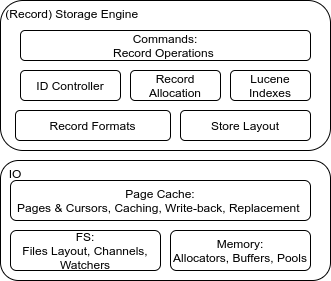
\includegraphics[keepaspectratio,width=0.5\textwidth]{img/N4J_Storage.png}
 \end{center}
 \caption{A visualization of the broad the storage and memory organization of Neo4J.} %TODO citation
\end{figure}

In the next section the focus is set on the storage layer of Neo4J: How it handles allocations, read and writes and how it provides the notion of a page. After that I elaborate on the details of the page cache, the transformation it applies to nodes and relationships on loading, the caching and the page eviction strategies it employs. Finally the internals of the files and records layouts are discussed along with the special structures employed and the indexes that are (or may be ) created over the files.


\section{Disk Space Management}
\mintinline{bash}{
neo4j/community/io/src/main/java/org/neo4j/io/fs/
} \\

\mintinline{bash}{neo4j/community/storage-engine-api/src/main/java/org/neo4j/storageengine/api/} \\

\mintinline{bash}{neo4j/community/native/src/main/java/org/neo4j/internal/nativeimpl/LinuxNativeAccess.java} \\

\href{Hpw delete works}{https://neo4j.com/developer/kb/how-deletes-workin-neo4j/} \\

\href{G-Store}{http://g-store.sourceforge.net/th/index.htm} \\

\href{Algorithms \& data structures}{https://www.youtube.com/watch?v=NlT21Ceg3y0}  \\

\href{Reusing space}{https://neo4j.com/docs/operations-manual/current/performance/space-reuse/\#space-reuse} \\



\section{Buffer Management}
% TODO use michael brendles work
\mintinline{bash}{
neo4j/community/io/src/main/java/org/neo4j/io/pagecache
}

\href{Page Cache layout ??? Outdated ???}{https://www.slideshare.net/thobe/an-overview-of-neo4j-internals} \\


\section{File, Record \& Index Structures}
    \subsection{Nodes}
    The record format of nodes consist of a 15 byte structure. The IDs of nodes are stored implicitly as their address. If a node has ID 100 we know that its record starts at offset 1500 from the beginning of the file. The struct of a record looks like this:
    \begin{enumerate}
     \item[Byte 1] The first byte contains the in-use flag .
     \item[Bytes 2 - 5] The next 4 Bytes represent the ID of the first relationship in the linked list containing the relationships of the considered node.
     \item[Bytes 6 - 9] Again 4 bytes encode the ID to the first property of the node.
     \item[Bytes 10 - 14] This 5 byte section points to the labels of this node, labels might also be inlined.
     \item[Byte 15] The last byte is reserved for aditional flags.
    \end{enumerate}
    This seems to be aligned with the following types. Taken from a comment from the source code:
    \mintinline{Java}{// in_use(byte)+next_rel_id(int)+next_prop_id(int)+labels(5)+extra(byte)}. \\
    
    \begin{figure}[htp]\label{node_layout}
    \begin{center}
    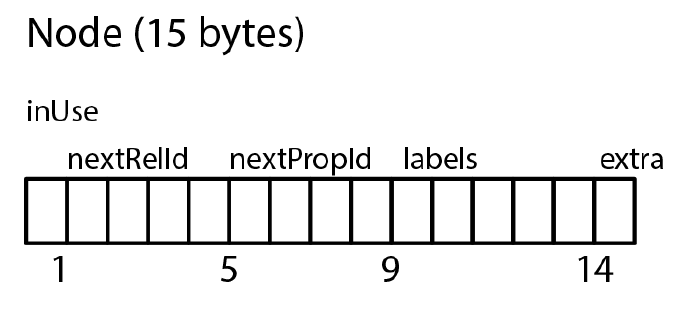
\includegraphics[keepaspectratio,width=\textwidth]{img/node_layout.png}
    \end{center}
    \caption{A visualization of the broad the storage and memory organization of Neo4J.} %TODO citation
    \end{figure}
    
     But also the sizes seem to be odd in some sense when looking at the definition of the maximal address sizes. Also from the source code:
     \begin{minted}{Java}
        public static final int PROPERTY_TOKEN_MAXIMUM_ID_BITS = 24;
        static final int NODE_MAXIMUM_ID_BITS = 35;
        static final int RELATIONSHIP_MAXIMUM_ID_BITS = 35;
        static final int PROPERTY_MAXIMUM_ID_BITS = 36;
        public static final int DYNAMIC_MAXIMUM_ID_BITS = 36;
        public static final int LABEL_TOKEN_MAXIMUM_ID_BITS = 32;
        public static final int RELATIONSHIP_TYPE_TOKEN_MAXIMUM_ID_BITS = 16;
        static final int RELATIONSHIP_GROUP_MAXIMUM_ID_BITS = 35;
        public static final int SCHEMA_RECORD_ID_BITS = 32;
     \end{minted}
    To summarize: The records on disk are stored as in the enumeration above. In the database all IDs get mapped to long and their respective space is larger than the space representable by 4 byte integers. This means in between there needs to be some rearrangements, to be investigated.
    
    \subsubsection{Node Labels}
    

    \subsection{Relationships}
    \begin{enumerate}
     \item[Byte 1] In-use flag 
     \item[Bytes 2 - 5] first node ID 
     \item[Bytes 6 - 9] second node ID 
     \item[Bytes 10 - 13] relationship type 
     \item[Bytes 14 - 17] previous relationship ID for first node
     \item[Bytes 18 - 21] next relationship ID for first node
     \item[Bytes 22 - 25] previous relationship ID for second node
     \item[Bytes 26 - 29] next relationship ID for second node
     \item[Bytes 30 - 33] link to the first property of the relationship
     \item[Bytes 34] next relationship ID for first node
    \end{enumerate}

    \begin{figure}[htp]\label{rel_layout}
 \begin{center}
  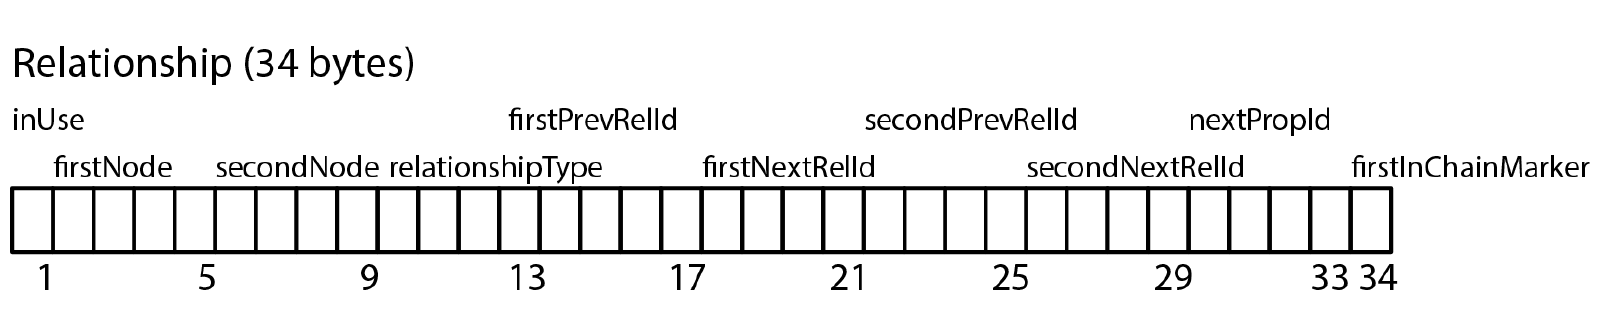
\includegraphics[keepaspectratio,width=\textwidth]{img/relationship_layout.png}
 \end{center}
 \caption{A visualization of the broad the storage and memory organization of Neo4J.} %TODO citation
\end{figure}
    
    \begin{minted}{java}
    // record header size
    // directed|in_use(byte)+first_node(int)+second_node(int)+rel_type(int)+
    // first_prev_rel_id(int)+first_next_rel_id+second_prev_rel_id(int)+
    // second_next_rel_id+next_prop_id(int)+first-in-chain-markers(1)
    \end{minted}
    
        \subsubsection{Relationship Types}
        \subsubsection{Relationship Groups}

    \subsection{Properties}
    \begin{enumerate}
     \item 
    \end{enumerate}
    
    \subsubsection{Strings \& Arrays}
    
    
    \subsection{Others}
        \subsubsection{Schema}
        \subsubsection{Metadata}

\mintinline{bash}{neo4j/community/record-storage-engine/.../kernel/impl/store/record/}

\mintinline{bash}{neo4j/community/record-storage-engine/src/main/java/org/neo4j/kernel/impl/store/} \\

\href{Layout N4J}{https://neo4j.com/developer/kb/understanding-data-on-disk/} \\

Ancient: \href{Slides: Internals Of N4J}{https://www.slideshare.net/thobe/an-overview-of-neo4j-internals} \\
\href{Video}{https://skillsmatter.com/skillscasts/2968-neo4j-internals} \\

\href{N4J Arch blog}{http://key-value-stories.blogspot.com/2015/02/neo4j-architecture.html} \\

\href{Followup discussion w devs}{https://groups.google.com/g/neo4j/c/cxClivwF94k}






\section{Example}
% TODO adapt from Brendle

\section{Conclusion}
The overall memory and storage state of a Neo4J instance and its environment may thus be visualized like this figure~\ref{N4J_memory_view}.

\begin{figure}[htp]\label{N4J_memory_view}
 \begin{center}
  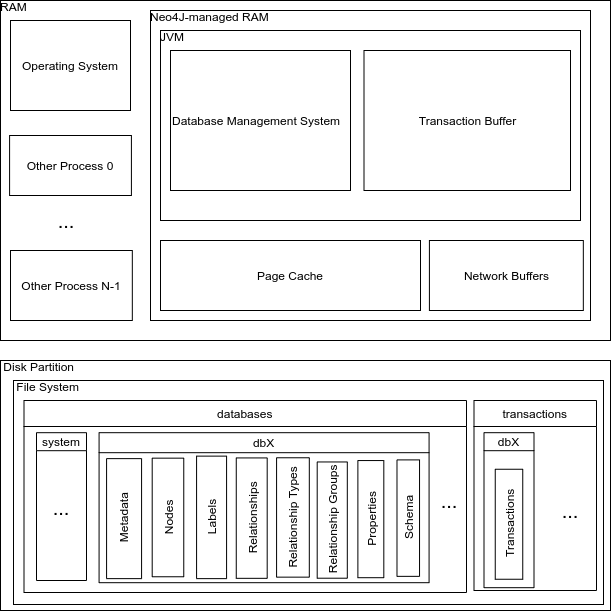
\includegraphics[keepaspectratio,width=\textwidth]{img/N4J_memory_view.png}
 \end{center}
 \caption{A visualization of the broad the storage and memory organization of Neo4J.} %TODO citation
\end{figure}

\end{document}
